\documentclass[12pt]{article}
\usepackage[utf8x]{inputenc}
\usepackage{graphicx} 		% Used to for importing images
\usepackage{indentfirst}	% Indents 1st paragraph (by default its off)
\usepackage{longtable} 		% Tables than can span over multiple pages
\usepackage{placeins}		% Used to keep images in place(via \FloatBarriers)
\usepackage{caption}		% Used to caption tabular 
\usepackage{amsmath}		% Dat math businezz
\usepackage{algorithm}
\usepackage[titletoc, title]{appendix} % Helps with appendix name formatting
\usepackage[hidelinks]{hyperref} % Used to create hyperlinks
\usepackage[nottoc,numbib]{tocbibind}

% Define Global Variables
\setlength{\parindent}{20pt}

\begin{document}

\begin{titlepage}

% Defines a new command to draw horizontal lines
\newcommand{\Line}{\rule{\linewidth}{0.5mm}} 

% Center everything on the page
\center
 
% textsc - capitalizes every letter
\textsc{\LARGE University of Gothenburg}
% Define gap after text line
\\[3.5cm] 

% Course code and name
\textsc{\Large DIT168}\\[0.3cm]
\textsc{\large Project: Industrial IT and Embedded Systems}\\[0.5cm]

% Use the defined command to draw lines
\Line \\[0.4cm]
{\huge \bfseries Final Report}\\[0.4cm]
\title{Final Report} % Line used to let overleaf automatically name the project
\Line \\[0.5cm]
 
% Large italic text
\Large \textit{Authors:}
\\Erik Laurin
\\Isabelle Törnqvist
\\Joacim Eberlen
\\Justinas Stirbys \\[3cm]

% Original date for the report
{\large Group 01} \\[0.3cm]
{\large https://github.com/justasAtGU/dit168} \\[0.3cm]
{\large \today}

% Fills the remaining page with whitespace
\vfill

\end{titlepage}

% Creating table of contents
\tableofcontents
\pagebreak

%%%%%%%%%%%%%%%%%%%%%%%%%%%%%%%%%%%%%%%%%%%%%%%%%%%%%%%%%%%%%%%%%%%%%%%%%%%%%%%%%%
% Project organization
%%%%%%%%%%%%%%%%%%%%%%%%%%%%%%%%%%%%%%%%%%%%%%%%%%%%%%%%%%%%%%%%%%%%%%%%%%%%%%%%%%
\section{Project Organization (by Erik)}\label{project organization}
In the inception phase of the project, the development team established the work process to be used throughout the project and whom would take on certain project roles. The team appointed Isabelle Törnqvist as testing manager, Justinas Stirbys as V2V manager and scrum master and Joacim Eberlen as the quality manager. Erik Laurin was given a  general role with no particular additional responsibilities.

The development team agreed to use the Scrum framework tailored with a few practices of the team's liking. At the start of each sprint, a sprint planning meeting was held ensuring that all team members had a shared uniformed vision. Meetings were scheduled twice a week, yet it quite quickly became evident that this was not enough and the development team started to meet more often. Stand-ups were executed daily (through Slack in case of no physical meeting). Furthermore, GitHub’s pull requests were used as a means of code review before merging into the master branch. GitHub issues were incorporated in the work process to report bugs and list other concerns that somehow had to be addressed by the developers. Lastly, retrospectives were carried out after each sprint to ensure that the developing team learnt from both potential shortcomings and things that went particular well.
 
The Figure \ref{fig:ganttchart} in Appendix \ref{appendix: figures} depicts the development team’s initial plan and how they managed to adhere to such. Note that the two activities marked with the Asterisk(*), were not included in the initial plan but added at a later stage. 

In addition, the ‘Ultrasonic’ activity did not only exceed the deadline but is still at 75 \% completion where it was abandoned. Reason being was difficulties in encapsulating required libraries in a Docker image (see section \ref{deployment issues} for additional details) and that a fully working image was provided that did exactly what the Ultrasonic activity was trying to accomplish. Consequently, resources in terms of manpower was relayed into more urgent matters. Furthermore, the same challenge was faced with the IMU, difficulties in encapsulating required libraries in the Docker image, which resulted in the IMU activity to fall behind schedule. 

The team chose to control the miniature car through a web-interface accessible to anyone connected to the vehicle. Through the incremental nature that Scrum promotes, the web-interface was expanded to visualize all data communication relying on the libcluon library\cite{libcluon}. Both the remote controller and the data visualization functionalities were fully functional and presented in week 15 and 16 respectively, thus according to plan. However, the team refined the web-interface with minor visual adjustments until it was deemed complete during week 17 (see the green markings in the chart).
\pagebreak

%%%%%%%%%%%%%%%%%%%%%%%%%%%%%%%%%%%%%%%%%%%%%%%%%%%%%%%%%%%%%%%%%%%%%%%%%%%%%%%%%%
% Conceptual ideas of all algorithmic aspects 
%%%%%%%%%%%%%%%%%%%%%%%%%%%%%%%%%%%%%%%%%%%%%%%%%%%%%%%%%%%%%%%%%%%%%%%%%%%%%%%%%%
\section{Conceptual Ideas (by Isabelle)}\label{conceptual ideas}
This section presents the conceptual ideas, as well as describing the fundamental functional aspects of the project.

The goal of this project was to develop a miniature smart vehicle with features that would allow it to form a platoon with similar vehicles. 

These features being:
\begin{itemize}
  \item The vehicle being remote controlled when in the role of a leader vehicle.
  \item A web-interface that shows intercepted messages from the internal and external OD4 sessions.
  \item Maneuvering logic that allows the car to act as a follower in a platoon.
  \item Ultrasonic sensor and corresponding logic that gives the vehicle collision control.
  \item Making use of an Inertial Measurement Unit (IMU) to derive the vehicle's heading and speed. 
\end{itemize}

In order to develop the platooning, the project teams were provided existing microservices for motor control, steering and ultrasonic readings. 

One of the fundamental requirements of this project is for the internal - as well as the external communication between vehicles - to make use of libcluon\cite{libcluon}.

The concept behind the remote controller was to have it in the same web-interface where the messages are being visualized. This was to ensure the usability for the driver of the car. The messages being visualized are intercepted messages from the internal and external communication channels. The interface should also host visualizations of the vehicles heading and speed, as well as a controller for leader/follower mode toggling.   

The idea was to use the IMU readings to derive the car's location and broadcast to following cars, but this concept was later scrapped due to unreliable readings of the speed, as well as inconsistencies in communication with other miniature vehicles development teams.  More specifically, it was scrapped, due to most teams failing to filter out the noise causing the IMU readings to become unreliable. During discussions on W17 with the teams, the project group presented following with, a consensus was reached to use PedalPositionReading and GroundSteeringAngle for following. Thus, by sending the IMU readings the development team would hinder interoperability and the quality of following. Moreover, the use of sending heading data as requested by one of the platooning teams, was scrapped by the other team, without a provided reason.
\subsection{Communication} 
The communication shown Figure \ref{fig:logical_view} is done using the libcluon\cite{libcluon} library. The library provides threaded and distributed messaging via OD4 Session objects, which in terms require an identifier to function. The identifier is denoted as a "CID" and is used for the purpose of specifying which channel to send or receive the message to/on. Every microservice, at the least has 1 class with a running OD4 sessions used to communicate to the the internal channel for the purpose of sending messages such as ultrasonic and IMU readings. Moreover, UDP Sender and Receivers, provided by the library, are used to communicate between project groups car, commonly known as Dash, and other cars. The only class containing UDP Senders and Receivers is the "v2v-protocol" as external and internal communication is the purpose of the class.
\subsection{Functional Requirements}
Functional requirements were defined by the project team based on the scope provided by the product owners. Provided in this section are the requirements deemed relevant for the conceptual idea of this project. The full list of requirements can be found in the SAD document \cite{SAD} located in the project's Git repository. 

\begin{longtable}{| p{0.05\linewidth} | p{0.15\linewidth} | p{0.45\linewidth} | p{0.25\linewidth} | p{0.1\linewidth} |}\hline 
    ID & Requirement & Description & Status & Priority \\ \hline
   	F1 & Message Log & A web page must contain a message log of everything that has been sent internally and externally within the car & Implemented & Must\\ \hline
   	F2 & Remote Controller & A web page must contain a graphical remote controller that communicates and controls Dash, when the car is the leader of the platoon & Implemented & Must\\ \hline
   	F4 & Leader Connection & The car, Dash, must be able to support Leader functionality (i.e. send LeaderStatus requests) while platooning & Implemented & Must\\ \hline       
    F5 & Follower Connection & The car, Dash, must be able to participate in platooning as a follower & Implemented & Must\\ \hline
    F6 & Maneuvering & The car will drive forward, turn left or right on commands received over the OD4 session & Implemented & Must\\ \hline
   	F7 & IMU & Dash must be able to use the IMU on its BeagleBoard Blue to calculate the distance moved & Implemented & Must\\ \hline
   	F8 & V2V Protocol & The car must be able to support the V2V Protocol. It is required for it to communicate with other cars and send sensors data & Implemented & Must\\ \hline
   	F9 & Collision Prevention & Dash will stop/brake when ultrasonic readings return an object that is less or equals to 10 cm ahead &  Implemented & Should\\ \hline
   	F10 & Emergency Brake & The car will stop if it fails to receive 3 update requests (i.e. hasn’t received anything in 300ms) and/or the connection to other cars has been lost & Implemented & Must\\ \hline
    \caption{Functional requirement specification table}
\label{tab:RequirementsT}
\end{longtable}
In this paragraph, the functional requirements will be referenced to by their ID, as specified in the table above. For the class diagram of the conceptual idea structure, please refer to figure~\ref{fig:logical_view}.  

The F1 and F2 requirements are both realized in the web-interface. "v2v-protocol" is the class where requirements F4, F5  and F8 are implemented. Requirement F7 is met in the "IMU" structure. The IMU readings are visualized in the web-interface, however due to reasons outlined in section \ref{integration issues}, the readings are not being sent via the V2V Protocol.

Finally, requirements F6, F9 and F10 are implemented and met in the maneuvering class. 

% Adding image
\FloatBarrier % -> Surround image with this, to make sure text does not wrap
\begin{figure}[ht!]
\centering
% Make image as wide as the line
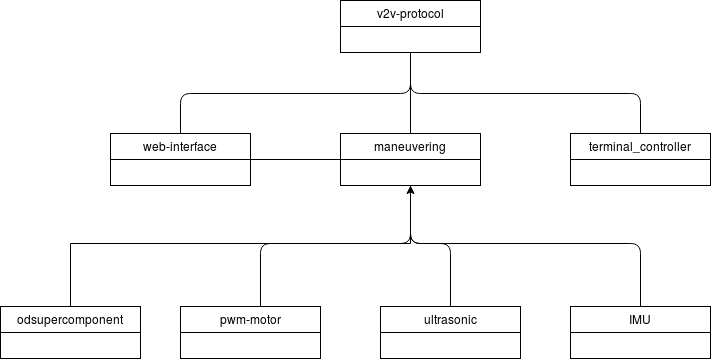
\includegraphics[width=\linewidth]{Figures/logical_view.png}
\caption{Class Diagram}
\label{fig:logical_view}
\end{figure}
\FloatBarrier % -> Surround image with this, to make sure text does not wrap
\subsection{Activity Diagram}   
Shown below is an activity diagram, to further explain how the concepts for this project were implemented. This describes the dynamic aspects of the conceptual idea in general terms. 

% Adding image
\FloatBarrier % -> Surround image with this, to make sure text does not wrap
\begin{figure}[H]
\centering
% Make image as wide as the line
\includegraphics[width=\linewidth]{Figures/ActivityDiagram.png}
\caption{Activity Diagram}
\label{fig:activitydiagram}
\end{figure}
\FloatBarrier % -> Surround image with this, to make sure text does not wrap
\pagebreak

%%%%%%%%%%%%%%%%%%%%%%%%%%%%%%%%%%%%%%%%%%%%%%%%%%%%%%%%%%%%%%%%%%%%%%%%%%%%%%%%%%
% Necessary algorithmic fundamentals
%%%%%%%%%%%%%%%%%%%%%%%%%%%%%%%%%%%%%%%%%%%%%%%%%%%%%%%%%%%%%%%%%%%%%%%%%%%%%%%%%%
\section{Algorithmic Fundamentals}\label{algorithmic fundamentals}
This section gives a deeper insight into the algorithmic fundamentals of the source code in the microservices maneuvering, IMU and ultrasonics.

\subsection{Maneuvering (by Erik)} \label{Maneuvering}
The microservice maneuvering acts as a hub connecting the microservices web-interface and v2v-protocol to the microservices that make the miniature car move. 
\par

The software developed had to enable the car to act both as a leader and a follower. Through the car’s web-interface, one can easily change the mode of the car between just following and leading. The mode request is sent to the maneuver microservice, see the state machine diagram below which illustrates the different modes (states).

 % Adding image
\FloatBarrier % -> Surround image with this, to make sure text does not wrap
\begin{figure}[ht!]
\centering
% Make image as wide as the line
\includegraphics[width=\linewidth]{Figures/StateMachineManeuvering.png}
\caption{State Machine Diagram - changing of mode}
\label{fig:STM_maneuvering}
\end{figure}
\FloatBarrier % -> Surround image with this, to make sure text does not wrap

As shown in the diagram above, the car's default setting, thus the mode the miniature car is in when starting, is leading. Consequently, in order for the following mode to be triggered, such must be done by the user through the web-interface. The sequence of events happening when changing mode can be observed as the first chain of events in the sequence diagram below.
% Adding image
\FloatBarrier % -> Surround image with this, to make sure text does not wrap
\begin{figure}[ht!]
\centering
% Make image as wide as the line
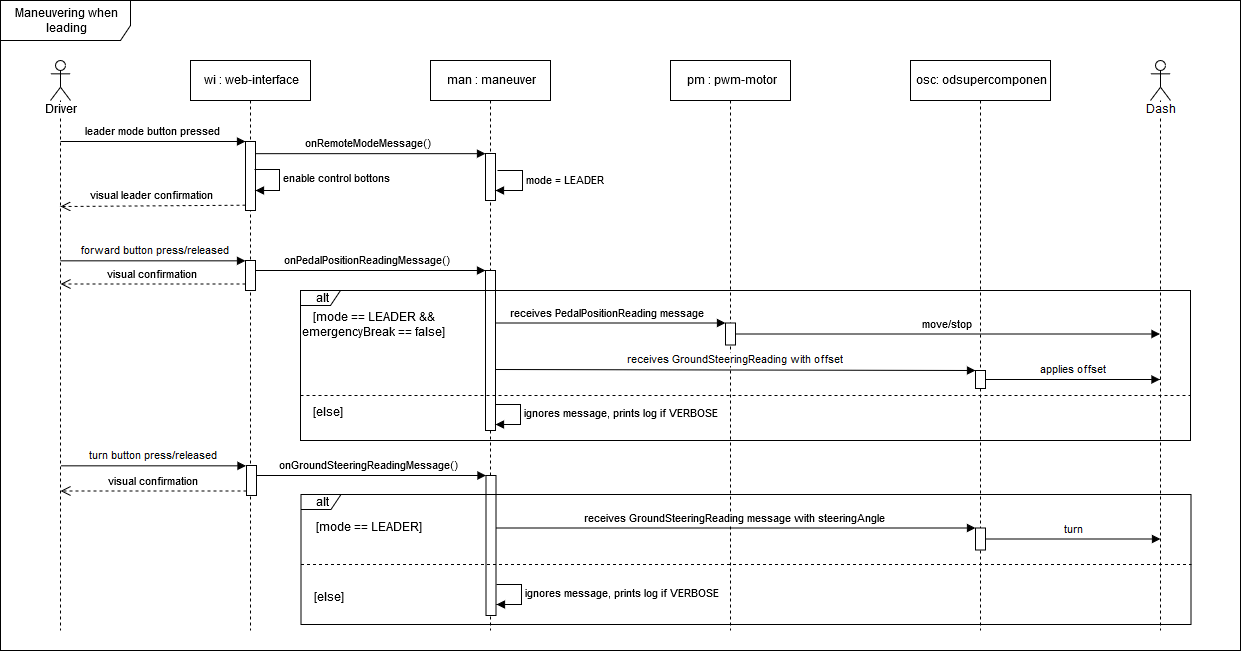
\includegraphics[width=\linewidth]{Figures/SequenceDiagramsManeuveringLeader.png}
\caption{Sequence Diagram - Leader}
\label{fig:SD_maneuvering_leader}
\end{figure}
\FloatBarrier % -> Surround image with this, to make sure text does not wrap

The diagram above depicts the chain of events when controlling the car through the web-interface. Note that turn and forward buttons can be pressed without any particular order. However, leading mode must be enabled for the microservice to evaluate the commands. In case leading mode is enabled and emergencyBreak is false (true in case an obstacle is detected by ultrasonic sensor within a specified distance), commands to move or stop will be forwarded to the pwm-motor microservice. In addition, to account for the car's drift, an offset is sent simultaneous as with aforementioned commands, see \ref{hardware issues} for details as to why. Lastly, commands to turn the servo and thus the car is directly forwarded to the odsupercompontent as long as leading mode is activated.

% Adding image
\FloatBarrier % -> Surround image with this, to make sure text does not wrap
\begin{figure}[ht!]
\centering
% Make image as wide as the line
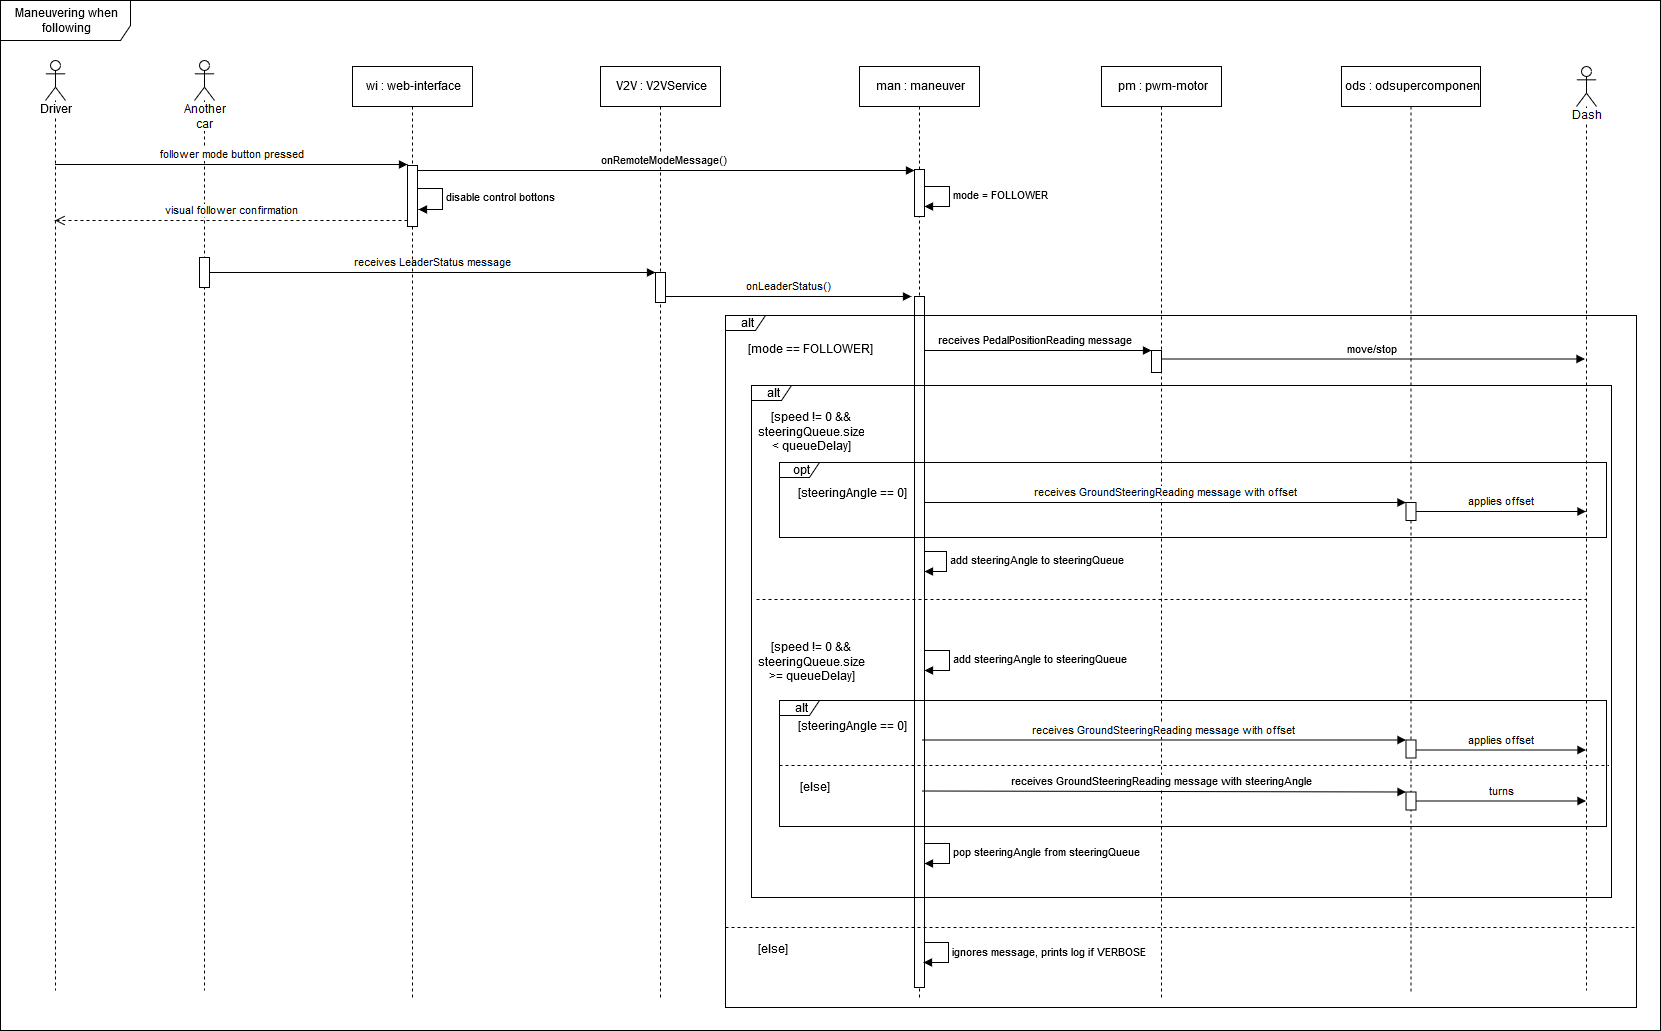
\includegraphics[width=\linewidth]{Figures/SequenceDiagramsManeuveringFollower.png}
\caption{Sequence Diagram - Follower}
\label{fig:SD_maneuvering_follower}
\end{figure}
\FloatBarrier % -> Surround image with this, to make sure text does not wrap

Similarly to the first sequence diagram, the diagram above illustrates the chain of events when the car is executing commands. However, instead of having a driver controlling the miniature vehicle directly through the web-interface, the car is following another miniature car autonomously. This is made possible through the retrieval of so called 'LeaderStatus' messages from the leading vehicle. This message is evaluated and processed and eventually a command is sent to the microservices odsupercomponent and pwm-motor for the car to move.

\pagebreak

\subsection{IMU (by Joacim)}

% Adding image
\FloatBarrier % -> Surround image with this, to make sure text does not wrap
\begin{figure}[ht!]
\centering
% Make image as wide as the line
\includegraphics[width=\linewidth]{Figures/SequenceDiagramIMU.png}
\caption{Sequence diagram IMU}
\label{fig:sd_imu}
\end{figure}
\FloatBarrier % -> Surround image with this, to make sure text does not wrap

The microservice has three classes, one for the IMU, one for the yawDegrees and one for acceleration. The IMU class handles the execution flow of the program, explained in this sequence diagram. The yawDegrees class gives us the current heading of the car in degrees, this is explained in section \ref{IMU section}.

When the IMU microservice is enabled the first action executed is starting the OD4 Session. When continuing, a statement to make sure the OD4 session is running. If not, the program throws an error telling the user that the OD4 session is not running. When the session is running we initialize the Robotics Cape library\cite{robotics cape} using initialize method. Afterward, the loop starts and runs until the OD4 session dies, the program then reads the hardware components using the Robotics Cape's reading functionality.  

If there are no errors in execution, the getHeading method is run. This method returns the current heading as a float value. The getHeading method is included in the yawDegrees class, it includes calculations to make sure the hardware component returns the correct value. 
To store the returned value readingSteergingAngle method is executed, it stores the value as a message for the OD4 session.

The getDistanceTravelled method is similar to the previous method, the call is to the acceleration unit of the car. The acceleration class calculates the current acceleration of the car in the physical realm.  The data is stored, as an OD4 ready message, using the getDistanceTravelled method.

The last step in execution is sending the values using the OD4 session we initialize at the beginning of the program.  

\subsection{Ultrasonics (by Joacim)}
The ultrasonic microservice, as seen in Appendix \ref{appendix: figures}, Figure \ref{fig:sd_ultrasonics} is a simple implementation to read the value and change the configuration of the hardware component. It uses the readUltrasonics method to get the data to create a message for the internal OD4 session. To set up the ultrasonics it is needed to change some setting on the hardware, which can be done using writeUltrasonics method. 

The activity starts by declaring an OD4 session and then making sure it runs properly. If not an error is thrown, to make sure the user knows there is something wrong. The gist of the microservice is, setting up the configuration for the ultrasonics based on command line arguments. Then reading the ultrasonic values in a loop, packaging them into OD4 ready messages and then sending in every iteration. 

\pagebreak

%%%%%%%%%%%%%%%%%%%%%%%%%%%%%%%%%%%%%%%%%%%%%%%%%%%%%%%%%%%%%%%%%%%%%%%%%%%%%%%%%%
% Source code implementation
%%%%%%%%%%%%%%%%%%%%%%%%%%%%%%%%%%%%%%%%%%%%%%%%%%%%%%%%%%%%%%%%%%%%%%%%%%%%%%%%%%
\section{Implementation Details}\label{implementation details}

The following section will showcase a selection of source code snippets and their implementation details to  further improve the understanding of algorithmic aspects. 
\par

\subsection{Maneuvering (by Erik)}
As mentioned in section \ref{Maneuvering}, the maneuvering microservice enables the miniature vehicle to be controlled by our software stack. The microservice acts as an intermediate step between the two OD4 session channels that are running on the vehicle. The internal OD4 channel carries messages from all microservices (but the odsupercomponent and pwm-motor), thus messages from both the web-interface and the V2V service are broadcasted on the internal channel. The other channel, the so called 'od4PwmOds', has the two microservices which are interfacing with the vehicle's servo and motor (odsupercomponent and pwm-motor) constantly listening for PedalPositionReading and GroundSteeringAngle messages, which make the car move. 

Maneuvering's source code makes use of libcluon's function dataTrigger, which carries out a predefined function on receive of a particular message on a particular channel (the internal OD4 channel in this case). Depending on which mode the car is set to when a message is received, different actions will be executed.

\subsubsection{onPedalPositionReading}
Figure \ref{fig:onPedalPositionReading_snippet}, Appendix \ref{appendix: figures}, shows a code snippet from Maneuvering.cpp, the script running in the Mneuvering microservice. The code depicts the function that gets executed when a PedalPositionReading message is received. The software stack includes an ultrasonic microservice, which broadcasts distance-to-obstacle readings to the internal OD4 channel. In case the reading is below the minimum breaking distance (is set as a command line argument when running the microservice), emergencyBreak will be set to true in the Maneuvering script and the function onPedalPositionReading will terminate immediately when called (see line 150). Consequently, the miniature car will not move forward when the the emergency break is applied. If the emergency break, however, is false, and the mode is set to leader, the PedalPositionReading message is forwarded to the pwm-motor microservice (see line 171) and the vehicle will move. Note that on line 169, a steering request, the offset, in the form of a GroundSteeringAngle message, is sent to the odsupercomponent to account for the vehicle's drift. Similarly to the PedalPositionReading message, which is forwarded directly when received on the internal channel to the 'od4PwmOds', is the GroundSteeringAngle message which also is forwarded to an appropriate microservice when received in maneuvering. See Figure \ref{fig:SD_maneuvering_leader} above for a sequence diagram that corresponds to the snippet.

\subsubsection{onLeaderStatus} \label{onLeaderStatus}
Another message that triggers a function to be called is 'LeaderStatus'. Such message is received when the vehicle is connected to another vehicle as a follower. The message contains, for instance, the leader vehicle's steeringAngleReading and PedalPostitionReading.

In Appendix \ref{appendix: figures} Figure \ref{fig:onLeaderStatus_snippet}, illustrating the onLeaderStatus function, on line 254, the speed from the LeaderStatus message is extracted and sent to the pwm-motor microservice on the following line. Hence, the vehicle will mimic the leading vehicle's motor commands, as soon as a  message of the aforementioned type is received. This resulted in a relatively seamless and rather accurate following behavior of the leader car when going  straight forward or stopping. 
\par
However, to get the car to follow in the leader car's tracks, the turning commands could not be executed directly on receive like the commands for going forward and stopping. To overcome this, the execution of turning commands are delayed. The approach for obtaining such behavior is using a queue and initially only recording commands, not executing them. In order for a car to turn, it must not only turn the wheels, but also go forward. Consequently, steering commands received together with a car speed of 0, will be ignored since such combination will not make the car move or turn. On line 258, the if-clause is entered if the speed received is not 0 and the queue, containing steering commands, is less than queueDelay. Inside the clause, the steering command is added to the steeringQueue. 

The clause on line 271 is entered if the speed received is not 0 and the size of the queue is equal, or greater, than the queueDelay. When these conditions are met, it is time for the script to start executing the old queued steering commands. After the addition of another steering command to the queue, the function followSteering is called and the very same queue is passed to it as an argument. The followSteering function executes the first steering command in the queue, through sending a GroundSteeringAngle message to the odsupercomponent microservice with the GroundSteeringAngle from the steering queue (as long as the steering command from the leader car is not 0, then the offset is sent instead). When this has been done, the steering command that was just executed is removed from the queue. See Figure \ref{fig:SD_maneuvering_follower} above for a sequence diagram that corresponds to the snippet.
\par
Consequently, by delaying the execution of the steering commands received from the leader vehicle, by using queueDelay to decide how many steering commands must have been received before the commands are executed, our vehicle, the follower vehicle, is able to mimic the leading vehicle's movements thus follow the vehicle. We chose to make queueDelay a variable that must be passed as a command line argument when starting the microservice, thus one is able to change the delay depending on current circumstances. For instance, latency between different network may vary greatly or the starting distance between the cars may differ. 
\par

\subsection{IMU (by Isabelle)} \label{IMU section}
The IMU class allows for access of the Inertial Measurement Unit (IMU) that is located on the vehicle. In this project, the 3-axis gyroscope and accelerometer included in the IMU were used to estimate the vehicle's speed, heading and distance travelled. 

The IMU source code made use of the Robotics Cape library\cite{robotics cape}, that was installed on the Beaglebone Blue. For further details, please refer to the knowledge acquisition documentation\cite{IMU} on the project's GitHub.  

The IMU class also makes use of libcluon \cite{libcluon}, in order to broadcast the estimated heading, speed and distance travelled to the internal OD4 session. 

\subsubsection{getHeading}
It is worth mentioning how the heading of the vehicle is calculated in this project. A 3-axis gyroscope, accelerometer and magnetometer were included in the IMU, and available for use in this project. However, due to the positioning of the IMU, the magnetometer's readings would be highly influenced by electronic currents, and was deemed unreliable. 

Instead, only the accelerometer and the gyroscope were used. Both measuring types comes with different drawbacks. An implementation of a complementary filter was used, fusing the readings of the accelerometer and gyroscope. As stated in the IMU knowledge acquisition: "The idea of sensor fusion is to get cleaner data, by canceling out the errors and weaknesses of the two types of sensors.

This implementation of a complementary filter high-passes readings from the fast and sensitive sensor, and low-passing data from the steady sensor, giving a result that is responsive in the short term while remaining accurate in the long term."\cite{IMU}

Figure \ref{fig:getHeading_snippet} shows a code snippet from yawDegrees.cpp, the code responsible for combining the accelerometer and gyroscope readings and calculating the vehicle's yaw, or heading. 

Line 35 and 36 shows the low pass and the high pass constants. 
For the reasoning for these constants, please refer to the knowledge acquisition documentation \cite{IMU}.

Line 37 shows how to get the steering angle using the accelerometer's proper acceleration readings in the two axes that exists in the 2D plane (the "x-axis" and "y-axis"). The reasoning behind using this to get $\theta$  is the assumption that the two readings could form the sides of a right-angled triangle. Using the basic trigonometric formula\cite{trigonometry} and law of tangents, $\theta$ can be derived from the accelerometer readings. 

The code on line 38 is the C++ implementation of this algorithm:
\begin{algorithm}                 
\caption{yaw in radius calculation using sensor fusion}    
		\[\theta = hpf\times(gyro\times \Delta t) + lpf\times acceldata\]
\end{algorithm}

$gyro$ being the angular velocity measured by the gyroscope. $\Delta t$, or deltaTime, in this implementation is the difference in time, meaning the sample time of which the IMU readings are collected.

Finally, code line 39-41 will convert the yaw result from radius to degrees, and round the decimals to a 0.01 value.  
\pagebreak

%%%%%%%%%%%%%%%%%%%%%%%%%%%%%%%%%%%%%%%%%%%%%%%%%%%%%%%%%%%%%%%%%%%%%%%%%%%%%%%%%%
% Software architecture
%%%%%%%%%%%%%%%%%%%%%%%%%%%%%%%%%%%%%%%%%%%%%%%%%%%%%%%%%%%%%%%%%%%%%%%%%%%%%%%%%%
\section{Software Architecture (by Joacim)}\label{software architecture}

\subsection{Component Section}
Deciding on architecture is a vital part of any project, thinking of what benefits a team can reap from the choice during the phases of development. During presentations by Dr. Rev. Christian Berger, it became quite obvious that their architecture of choice was microservices. The team had discussion about the pros and cons of this, see section \ref{microservice rationale}. 

One of the benefits of not choosing the microservice architecture was going for a more familiar architecture that the developers have experience working with. During early discussions, the development team did not find enough reason to not try the new way of designing the system.

% Adding image
\FloatBarrier % -> Surround image with this, to make sure text does not wrap
\begin{figure}[ht!]
\centering
% Make image as wide as the line
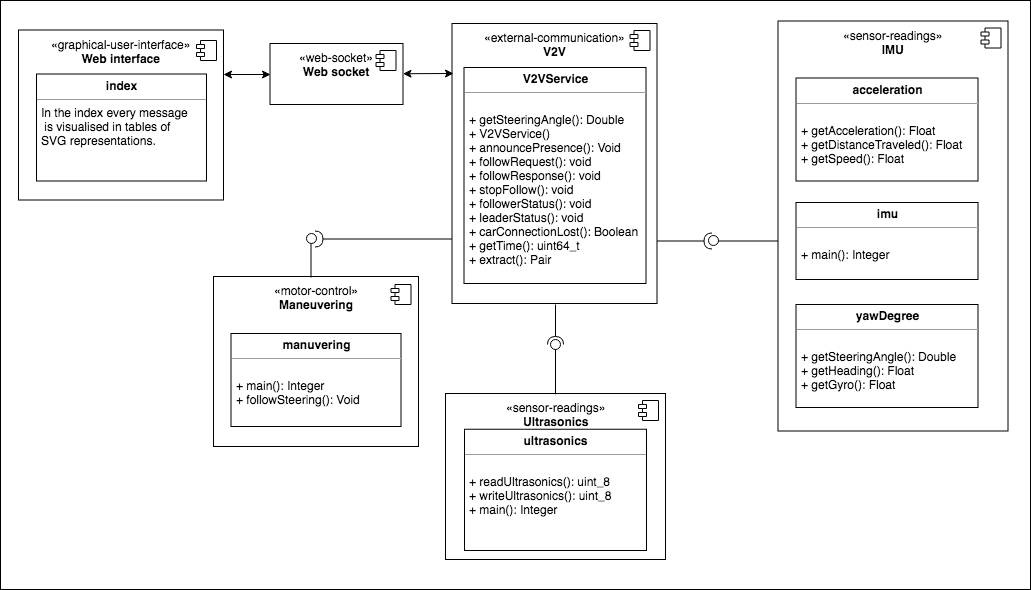
\includegraphics[width=\linewidth]{Figures/StructuredClassDiagram.png}
\caption{Structured class diagram}
\label{fig:Structured_class_diagram}
\end{figure}
\FloatBarrier % -> Surround image with this, to make sure text does not wrap

\subsubsection{V2V Service}
Designed with the V2V Service as a central node in our architecture we can easily route data throughout the system using different CID:s. The project uses multiple connection channels in the V2V Service:
\begin{enumerate}
\item Internal [Channel 122]
This channel is used by the system for internal communication. The internal channel was a design decision based on scalability of our system. Utilizing this channel every part of our system can easily access the data needed to visualize or execute actions accordingly.
\item Broadcasting [Channel 250]
This channel has some of the messages for the external systems in our environment. The external systems are composed out of other groups cars.  The message, at the moment of writing this,  using the channel is the announce presence. If there is a need to send more messages in this channel it can be developed further.
\item Incoming [UDP Connection]
This UPD connection reroutes the incoming messages from other vehicles into the internal channel. When the messages have been distributed, the rest of the system can use the Internal channel OD4 session to access this data. 
\item To Leader [UDP Connection]
This channel is used to send messages to the leader car. This is based on the V2V protocol that all groups use, the protocol gives us a straightforward implementation to exchange data between the cars. 
\item To Follower [UDP Connection]
The follower channel sends status updates to the follower car, the messages sent through this channel gives a uniform understanding of the current position of the cars of interest. 
\end{enumerate}

\subsubsection{IMU}
To use the IMU on the BeagleBone board some calculations were needed to be conducted. This microservice has the calculations of the returned data from the IMU hardware component.  

The IMU is used to get the change in heading, distance traveled and speed of the car. It broadcasts the data through an enveloped message to the internal channel. 
\subsubsection{Maneuvering}
The maneuvering microservice is the connection to the actual hardware of the car, it sends the messages from the V2V microservice to control the vehicle. It is designed with two modes, one follower, and one leader. The mode is supposed to decide what messages are interesting to the miniature car.
\subsubsection{Ultrasonics}
The ultrasonic microservice gives the distance in front of the car, it reads the values from the connected hardware component on the car. The rationale for this service was mainly the emergency brake event. The plan was to use a dynamic user-set distance, which should stop the car instantly. In the future, this could provide redundancy with other components to secure the execution of the emergency brake.
\subsubsection{Web Interface}
To control the car manually and visualize the internal working of the system, it was decided to use an extension of Chalmers Revere's signal viewer\cite{signal viewer}. In this microservice, we integrated the manual controls as arrow keys and divided the messages into internal and external, to make the visualization a bit clearer. The external messages are everything sent by the V2V Protocol, whereas the internal messages are the data transfered with the project group's vehicle. The IMU and the ultrasonic sensor is represented in animated images, this gives the user a better experience when using the system.  
\subsubsection{Terminal Controller}
As an interface for testing the car during the project, another microservice, the Terminal Controller, was used. It was developed for simplicity and stability. Initially, the web-interface was a bit lacking in performance and the terminal controller could be used as a backup. Having a backup microservice to use when needed increases the redundancy of the development process, but provides the system users with a backup remote controller that could be used for testing purposes and web-interface validation. 

\subsection {Rational for Microservices} \label{microservice rationale}

Using the aforementioned microservices when working with an embedded system that contains not only our own services, but also microservices created by other developers, gave us a more modifiable system. When microservices are paired with Docker or other operating-system-level virtualization techniques, the whole system becomes fully portable. Moreover, as a whole, a shared vision and knowledge sharing between developers was easier to convey. 

If the team were to continue developing the solution for the autonomous driving or graphical user interface this type of architecture has the power to scale seamlessly as an infinite number of additions can be developed with ease.

One of the bad things with the chosen architecture was, what should each of the services contain, how small should they be and how can we make sure there is no overlap in functionality in the system. In our case, the solution was partly to have a predefined process to ensure that aforementioned shortcomings were mitigated (see section \ref{project organization} for process details). Even if this process needed to be improved, the practice of dividing the work was carried over from earlier endeavours for the majority of our team. 

When pressed for time, a microservice based architecture can be a large benefit due to the enabling of parallel development of the different services. Anything developed should be able to run independently from everything else in the system. This gave us the ability to test, format and refine each service without having to worry about any other developers work progress. Delivering for each deadline during the project was uncomplicated to monitor, everyone knew who needed to do what part and could help accordingly.
\pagebreak

%%%%%%%%%%%%%%%%%%%%%%%%%%%%%%%%%%%%%%%%%%%%%%%%%%%%%%%%%%%%%%%%%%%%%%%%%%%%%%%%%%
%  Hardware/software integration
%%%%%%%%%%%%%%%%%%%%%%%%%%%%%%%%%%%%%%%%%%%%%%%%%%%%%%%%%%%%%%%%%%%%%%%%%%%%%%%%%%
\section{Hardware \& Software Integration (by Justinas)}\label{hardware software integration}
\subsection{Software Deployment}
For the purpose of hardware/software integration visualization a deployment diagram has been provided. As seen in Figure \ref{fig:deploymentdiagram} the software was deployed onto a BeagleBone. Most of the software developed was encapsulated within Docker images, with few exceptions, see section \ref{deployment issues}. \par

The communication between the microservices is done using OD4 Sessions provided by libcluon\cite{libcluon}, as such libcluon is either installed or included as a header only library in each microservice. Moreover, each microservice includes, at the minimum, a Messages.odvd file that defines message specification and an OD4 Session to transfer the readings to an internally defined OD4 channel, expressed with CID 122. \par
There exist 3 most notable hardware \& software integration examples; ultrasonics, IMU and the web-interface.\par

% Adding image
\FloatBarrier % -> Surround image with this, to make sure text does not wrap
\begin{figure}[ht!]
\centering
% Make image as wide as the line
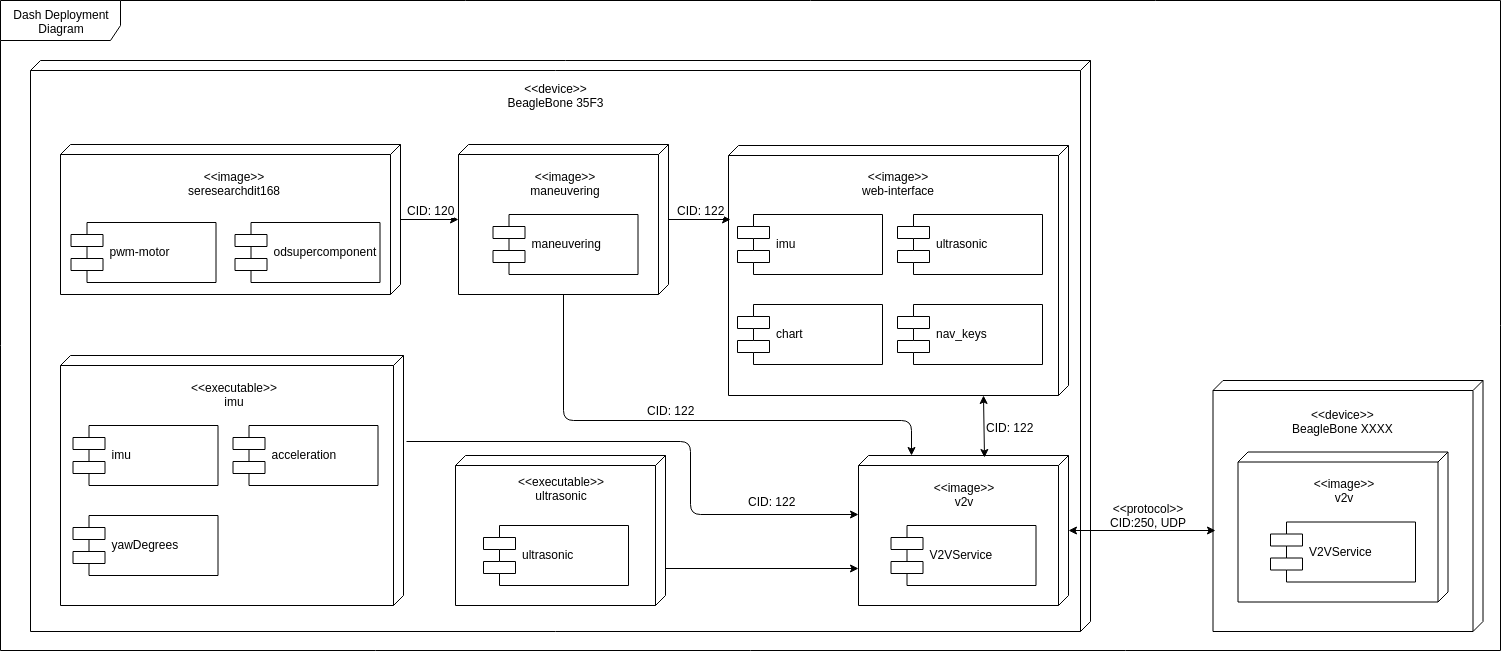
\includegraphics[width=\linewidth]{Figures/DeploymentDiagram.png}
\caption{Deployment Diagram}
\label{fig:deploymentdiagram}
\end{figure}
\FloatBarrier % -> Surround image with this, to make sure text does not wrap

\subsubsection{Ultrasonic \& IMU}
The "ultrasonic" and "imu" microservices both incorporate Robotics Cape\cite{robotics cape} library to interact with project's car, i.eDash's ultrasonic sensors and the IMU within the BeagleBone respectively. The readings are then sent packaged in a defined message to the internal communication channel, part of the "v2v" microservice. Moreover, since there are two provided ultrasonics, but only the front one is within the project, the ultrasonic microservice listens to a single specified hardware bus. 

\subsubsection{Web Interface}
The interface was developed using JavaScript, HTML and CSS, as such it uses libcluon.js. The web interface is responsible for both the remote controller and the data visualization. \par

The data visualization aspect of the interface is special in regards that it visualizes every message that miniature vehicle, Dash, receives or sends including hardware readings as indicated by the interface's software "imu" and "ultrasonic" components in Figure \ref{fig:deploymentdiagram}. The interface listens for messages incoming on the CID 122 channel before visualizing them. The "chart" component is used to create graphical representation of the messages. \par

The remote controller aspect of the interface consists of "nav\_keys" component. Once designated keyboard keys are pressed the commands to move are sent to the internal channel. From there the "maneuvering" microservice would intercept the messages on CID 122, the internal channel, and pass them to the microservices interfacing with the motor and servo, listening on CID 120. The reasoning behind this decision was to allow swapping between the leader and follower modes and applying an offset, discussed in section \ref{hardware issues}, without affecting the LeaderStatus that is being sent. Additionally, it is believed that with this approach, the channel dedicated for interfacing with microservices controlling the hardware actuators would not be filled with irrelevant messages.\par

\subsection{Integration Issues}\label{integration issues}
Integrating developed software with the given hardware proved to be more difficult than initially expected. The development team, Group 01, was faced with several integration issues while testing platooning with Groups 02 and 07, shown in Table \ref{issue table}, Appendix \ref{appendix: tables}. This section of the report is aimed to document and reflect on said issues.

\subsubsection{Hardware}\label{hardware issues}
Hardware issues showed to be the most prevalent and difficult to overcome. The most severe issue is considered to be IS1. The vehicle is physically able to turn right when a RC remote controller is directly connected to the servo. To combat this problem the team has taken the miniature vehicle to Johanneberg, talked with the course Teaching Assistant's, re-flashed to a newer BeagleBone image, and used PS4 controller image\cite{PS4 controller} to test turning right. These methods have been used to verify that the software was not faulty and as of yet the issue has not been resolved. \par
The second issue, IS2, emerged while testing remote controller software. The development team solved the problem by providing offset to compensate for the drift. The offset is applied only when the miniature is moving forward. \par
During platoon testing with Group 02 a the issue, IS4, emerged. The difference in acceleration speeds would cause Group 02's car, which acted as a follower, to fall behind the leader, the development team's car. Thus elongating the initial distance between the vehicles and failing to perform accurate platooning. The development teams had attempted to solve the issue by changing the vehicle configuration settings via a programming card. However, there was no difference between the acceleration settings. The real cause of the issue, proved to be a loosely tightened drive shaft on Group 02's miniature vehicle. The development team learnt to take into account the different miniature vehicle capabilities and hardware states while testing from that point on. \par
Issue IS3, appeared this time as well. Due to IS3, the IMU is only utilized for data visualization, it was not used for platooning implementation as initially planned, which caused the team to incorporate message based queue with PedalPositionReading and GroundSteeringAngle, see section \ref{onLeaderStatus} for more implementation details.  

While testing platooning with Group 07, with the development team acting as a leader for the other team. Another issue that presented itself was different vehicle turning capabilities, IS5. To accurately replicate the movements the development team had to lower it's turning angle, while Group 07 would double the angle they receive.

\subsubsection{Software Deployment}\label{deployment issues}
The Robotics Cape library\cite{robotics cape} provided a great number of difficulties when attempting to package software into Docker containers, IS6. A number of hours were wasted attempting to overcome this issue, with no success. The group decided to compile the software as an executable program on the car, as such shown in Figure \ref{fig:deploymentdiagram}. This approach was chosen, due to time constraints imposed by the project plan. To avoid falling behind and jeopardizing the project success, the team thought it would be more valuable to spend the time and resources on other activities, such as platooning realization. The microservices that failed to be encapsulated in Docker images include "imu" and "ultrasonic". \par

\subsubsection{V2V Protocol}
Platoon testing showed several V2V-Protocol pitfalls, relating to the established emergency scenarios. The agreed upon scenarios; vehicle stopping without crashing if the ultrasonics detect an object 10cm ahead, the vehicle stop following if it has not received a LeaderStatus/FollowerStatus in 375ms, proved to not work in practice, as the variables were set too low. The 10cm were not enough, due to the wheels of the car having insufficient grip. The 375ms were not enough, as the connection between the cars was still reliable and following with this variable would cause the cars to disconnect mid platooning. The issues IS7 \& IS8 are reflecting of these issues. \par

Moreover, when visualizing messages with no fields, libcluon would cause a parsing issue\cite{libcluon parse issue}, IS9. The parsing issue being caused by returning "\{\}" if no message field detected. The solution to this and the previously mentioned V2V pitfalls has protocol tailoring. The project group introduced a "status" field to avoid parsing errors, and the emergency scenario values were increased as seen fit by the groups presenting together. 
\pagebreak

%%%%%%%%%%%%%%%%%%%%%%%%%%%%%%%%%%%%%%%%%%%%%%%%%%%%%%%%%%%%%%%%%%%%%%%%%%%%%%%%%%
%  Description and results from the applied tests
%%%%%%%%%%%%%%%%%%%%%%%%%%%%%%%%%%%%%%%%%%%%%%%%%%%%%%%%%%%%%%%%%%%%%%%%%%%%%%%%%%
\section{Project Test Results (by Isabelle)}\label{project test results}
This section describes the testing that was done in the project.
\subsection{Manual Testing}
The majority of test performed in this project were of the manual type. The reason for this was a combination of two factors: the act of redundancy of testing a provided library \cite{libcluon}, which left little room to test the software being developed. The other aspect was that the results given from development were physical results, due to the product being embedded in hardware.

\subsubsection{V2V Communication}
There were two aspects to the V2V service: the following and the leading in a platoon. Both of these aspects were tested manually. Initially this was tested internally in the team, done mainly from computer to computer. Later, tests were done involving another development team, testing from car to car. 

It was while carrying out these manual communication tests that a threading issue was revealed. Previously, a single thread was responsible for both sending and receiving messages, resulting in the blocking of parallel executions. A need for a second thread was discovered, in order to send messages and receive messages simultaneously. Once a second thread was introduced, the issue was solved.   

\subsubsection{Maneuvering and Remote Controller}
The maneuvering was tested to some extent in combination with the remote controller. The other aspect was when Dash was being maneuvered as a follower vehicle. 

The conditions mentioned in Table \ref{tab:maneuverDT}, Appendix \ref{appendix: tables} consider both these aspects, as "sent" refers to input messages either from a a remote controller, or a leader vehicle that is being followed by Dash. 

\subsubsection{IMU}
The manual tests performed regarding the IMU are described in Table~\ref{tab:IMUDT}, Appendix \ref{appendix: tables}.

The preconditions for these tests were that the vehicle should be kept as parallel to the ground as possible. The IMU allows to detect pitch, roll and yaw. Meaning, it will detect angular velocity and proper acceleration in all 3 dimensions. However pitch and roll has not been accounted for in this implementation, and may effect the result of the yaw.

When testing the distance travelled, the travel surface is expected to be smooth and not inclined nor declined. 

\subsection{Unit Testing}
\subsubsection{IMU}
Unit tests were created for the IMU, as it was deemed useful to individually test the units where algorithms were located. 

The features tested were done so in a manner to verify that the functionality performed as intended. Meaning these tests were on the second maturity level on the Bezier testing scale\cite{BezierTestingLevels}. 

For writing the following unit tests, the test framework "catch"\cite{catchframework} was made use of. 

The two ways of calculating the vehicles heading were both tested in the unit test. 
The calculation for heading was tested both with sample values collected from manually testing of the vehicle, as well as "mock" values provided in Robotics Cape documentation\cite{robotics cape}.

The vehicles distance travelled, speed and acceleration were all tested with mock data as well. 

\subsection{Code Quality Verification}
Tools and certain conventions were utilized in this project to ensure a level of code quality. 

The source code verification tool vera++\cite{vera++} was used to analyse C++ code quality. The tool was used in combination with cmake, upon build. On encapsulation in a Docker image, the build would fail if criteria set by vera++ were not met.  This method of code quality verification was done in order to ensure readability of the C++ source code, as well as future maintainability. 

cppcheck\cite{cppcheck} was another tool that was used in combination with cmake. This static analysis tool was applied upon build for static analysis of the source code, and would fail the build if unwanted behavior was discovered.

The project team agreed to a convention in regards to developing source code, that states that warnings should be treated as errors. Again, the purpose of this convention was to ensure quality in the long run, and make sure the source code continues to be readable and maintainable.  

\subsection{Problematic Aspects} \label{test issues}
The purpose of this section is to address a few problematic aspects of the tests performed in this project. It may also be used as a pointer for improvement for future reference.

Worth mentioning is also the lack of test results and test reports. The team failed to carry tests out continuously, as well as document tests as they were performed. 

\subsubsection{Lack of Tests Performed}
The lack of tests for certain parts of the project was due to the extensive use of the provided library libcluon \cite{libcluon}. This library was not further developed by the project team concerned in this report. Because of this it was deemed redundant to write tests for developed software including the libcluon library.      

\subsubsection{Bezier Testing Levels}
The testing performed in this project stayed on the lower levels on the Bezier maturity scale. The testing was mainly manual ones, ad hoc and without much structure. Manual tests were not documented at the time of execution, and therefore not repeatable in a structured manner. Some tests met the standards of a level 2: testing and verifying that a feature works. 

\pagebreak

%%%%%%%%%%%%%%%%%%%%%%%%%%%%%%%%%%%%%%%%%%%%%%%%%%%%%%%%%%%%%%%%%%%%%%%%%%%%%%%%%%
%  Project’s retrospective
%%%%%%%%%%%%%%%%%%%%%%%%%%%%%%%%%%%%%%%%%%%%%%%%%%%%%%%%%%%%%%%%%%%%%%%%%%%%%%%%%%
\section{Project Evaluation (by Justinas)}\label{project evaluation}
The section aims to examine the overall project by providing focus on the aspects that went either exceptionally well or poorly. For a weekly, or sprint-wise, breakdown of the project refer to Sprint Retrospectives\cite{sprint retrospectives}.

\subsection{The Good}
Aspects of the project that went exceptionally well can be attributed to team organization, refer to section \ref{project organization}, and team dynamics. \par
It is believed, by the team, that all of the developers have contributed throughout the entirety of the project. The development team was able to meet all deadlines as defined by the course roadmap, including W17 Vehicle following. Although, admittedly the time based queue implementation is a bit disappointing, see section \ref{onLeaderStatus}. Moreover, the team had reasonably good communication as daily stand-ups would be used to notify others of problems encountered and as a way of asking for help. \par
The team's relationships played a significant part in improving the project. At no point in time, did the team have issues with any of its members not actively engaging during meetings or discussions, taking responsibility for their tasks or showing commitment to the project. However, this is not to say that there were no pitfalls with the project organization or that the quality and amount of engagement did not fluctuate throughout the project. \par

\subsection{The Bad}
Aspects that went poorly, as thought by the team, nearly all relate to project organization. \par
The initial two weeks after the acquisition of miniature vehicles, W13-14, went exceptionally bad. The development team was used to working in two week sprint increments followed by a sprint review. However, this was not imposed by the course as it provided more freedom. As such this caused the development team to momentarily abandon their process. It is believed that the Scrum Master should have enforced the defined process{ref to work process} more strictly during this period. \par  
Another aspect of project organization that could benefit from a vast improvement was knowledge sharing. The issue became apparent during W17, while testing with other teams, for specific integration issues, see section \ref{integration issues}. The issue caused certain team members to become critical failure points and others to lack the knowledge required to efficiently contribute for certain tasks. The issue could be solved by improving the amount of knowledge sharing in the project as well as conducting face-to-face code reviews on a defined basis. \par
Lastly, the final major issue is seen as a lack of tests, for testing issues see section \ref{test issues}. The issue is attributed to development team having a limited experience with testing. Moreover, as the library libcluon has done expansive testing and with everything being integrated and dependent with/on libcluon, this caused the team issues  with identifying aspects of the code to test as the tests could be seen as redundant.  

\subsection{And The External}
As a large portion of the project included inter-team cooperation for the development of the V2V-Protocol and platooning realization, an additional subsection focusing on V2V managerial matters was provided. \par
The most significant aspect that went well for the V2V-Protocol was it's early completion. Largely due to Julian Bock, the V2V manager from Group 5, and his contributions to the protocol. The early completion provided project groups with a large amount of time to test and tailor their versions of the protocol. Moreover, it reduced the amount of work needed to be carried out at later stages of the project. \par
On the other hand, it did not seem as though all the V2V managers had the same unified understanding of the protocol at later stages of the project. This includes some managers believing that the protocol was intended to work without making any modifications to it by their group. Moreover, the lack of shared vision amongst the managers caused some confusion surrounding message contents and how often some messages are required to be sent. To avoid said issues, the V2V managers should have spent more time ensuring that they were on the same page. \par 
Additionally, most of the V2V meetings suffered from inefficiency. Agendas were began to be made halfway through Study Period 2. To improve the V2V meeting efficiency agendas could have been made from the beginning.  \par
\pagebreak

%%%%%%%%%%%%%%%%%%%%%%%%%%%%%%%%%%%%%%%%%%%%%%%%%%%%%%%%%%%%%%%%%%%%%%%%%%%%%%%%%%
%  List of external references
%%%%%%%%%%%%%%%%%%%%%%%%%%%%%%%%%%%%%%%%%%%%%%%%%%%%%%%%%%%%%%%%%%%%%%%%%%%%%%%%%%
\def\refname{References} % Rename bibliography
\begin{thebibliography}{00}
	\bibitem{libcluon} Berger, C., libcluon, GitHub repository: \url{https://github.com/chrberger/libcluon}
	\bibitem{libcluon parse issue} Berger, C., libcluon, Lines 49-82, GitHub repository: \url{https://github.com/chrberger/libcluon/blob/75dd821002d2e14e76eb314a9e4b7078bf3b6a0d/libcluon/src/EnvelopeConverter.cpp}
	\bibitem{robotics cape} Strawson Design, Robotics Cape, Website: \url{http://www.strawsondesign.com/\#!}
	\bibitem{ultrasonics} Devantech, SRF08 UltraSonic Ranger, Link: \url{http://coecsl.ece.illinois.edu/ge423/DevantechSRF08UltraSonicRanger.pdf}
	\bibitem{catchframework} Catch Org, catch test framework, repository: \url{https://github.com/catchorg/Catch2}
	\bibitem{vera++} Vera Team, vera, repository: \url{https://github.com/verateam/vera}
	\bibitem{cppcheck} Cppcheck, url: \url{http://cppcheck.sourceforge.net/}
	\bibitem{trigonometry} Trigonometry, law of tangents, \url{https://en.wikipedia.org/wiki/Trigonometry}
	\bibitem{ComplementaryFilter} Malinen, E., "Fusion of Data from Quadcopter’s Inertial Measurement Unit Using Complementary Filter" \url{
https://www.doria.fi/bitstream/handle/10024/116099/IMU_data_processing_final.pdf?sequence=2}
	\bibitem{signal viewer} Chalmers Revere, GitHub repository: \url{https://github.com/chalmers-revere/opendlv-signal-viewer}
	\bibitem{PS4 controller} Chalmers Revere, PS4 controller, GitHub repository: \url{https://github.com/chalmers-revere/opendlv.miniature/tree/dit168/code/proxy-miniature/ps4controller}
	\bibitem{BezierTestingLevels} Bezier Testing Maturity Levels, url: \url{https://en.wikipedia.org/wiki/Testing_Maturity_Model}
\end{thebibliography}
\pagebreak

%%%%%%%%%%%%%%%%%%%%%%%%%%%%%%%%%%%%%%%%%%%%%%%%%%%%%%%%%%%%%%%%%%%%%%%%%%%%%%%%%%
% List of our referenced documentation
%%%%%%%%%%%%%%%%%%%%%%%%%%%%%%%%%%%%%%%%%%%%%%%%%%%%%%%%%%%%%%%%%%%%%%%%%%%%%%%%%%
\def\refname{Supporting Project Documentation} % Rename bibliography
\begin{thebibliography}{00}
	\makeatletter				% Needed to increase second bibliography index
	\addtocounter{\@listctr}{12}% Needed to increase second bibliography index
	\makeatother				% (Possibly) Needed to increase second bibliography index
	\bibitem{project repo} Laurin, E., Törnqvist, I., Eberlen, J., \& Stirbys, J., dashFTABs, GitHub Repository: \url{https://github.com/justasAtGU/dit168}
	\bibitem{v2v fork} V2V Managers, V2V-Protocol Link to fork: \url{https://github.com/justasAtGU/v2v-protocol}
	\bibitem{sprint retrospectives} Laurin, E., Törnqvist, I., Eberlen, J., \& Stirbys, J. Sprint Retrospectives, GitHub repository: \url{https://github.com/justasAtGU/dit168/tree/master/doc/SprintRetrospectives}
\bibitem{SAD} Laurin, E., Törnqvist, I., Eberlen, J., \& Stirbys, J. SAD, GitHub repository: \url{https://github.com/justasAtGU/dit168/blob/master/doc/Architecture}
\bibitem{IMU} Törnqvist, I., "Appropriate Algorithms and Adapting Available Concepts for IMU Regarding Acceleration and Yaw Calculation", repository: \url{https://github.com/justasAtGU/dit168/blob/master/doc/KnowledgeAcquisition/knowledgeAcquisitionIMU.pdf}
\end{thebibliography}
\pagebreak

%%%%%%%%%%%%%%%%%%%%%%%%%%%%%%%%%%%%%%%%%%%%%%%%%%%%%%%%%%%%%%%%%%%%%%%%%%%%%%%%%%
% Appendix of figures
%%%%%%%%%%%%%%%%%%%%%%%%%%%%%%%%%%%%%%%%%%%%%%%%%%%%%%%%%%%%%%%%%%%%%%%%%%%%%%%%%%
\begin{appendices} 
\section{Figures}\label{appendix: figures}
\begin{figure}[H]
\centering
% Make image as wide as the line
\includegraphics[width=\linewidth]{Figures/ganttchart.PNG}
\caption{Gantt Chart}
\label{fig:ganttchart}
\end{figure}

% Adding image
\begin{figure}[H]
\centering
% Make image as wide as the line
\includegraphics[width=\linewidth]{Figures/SequenceDiagramUltrasonics.png}
\caption{Sequence diagram ultrasonics}
\label{fig:sd_ultrasonics}
\end{figure}

% Adding image
\begin{figure}[H]
\centering
% Make image as wide as the line
\includegraphics[width=\linewidth]{Figures/yawDegrees_getHeading_snippet.PNG}
\caption{Code snippet - getHeading function}
\label{fig:getHeading_snippet}
\end{figure}

% Adding image
\begin{figure}[H]
\centering
% Make image as wide as the line
\includegraphics[width=\linewidth]{Figures/onLeaderStatus_snippet.PNG}
\caption{Code snippet - onLeaderStatus function}
\label{fig:onLeaderStatus_snippet}
\end{figure}

% Adding image
\begin{figure}[H]
\centering
% Make image as wide as the line
\includegraphics[width=\linewidth]{Figures/onPedalPositionReading_snippet.PNG}
\caption{Code snippet - onPedalPositionReading function}
\label{fig:onPedalPositionReading_snippet}
\end{figure}
\pagebreak

%%%%%%%%%%%%%%%%%%%%%%%%%%%%%%%%%%%%%%%%%%%%%%%%%%%%%%%%%%%%%%%%%%%%%%%%%%%%%%%%%%
% Appendix of tables and charts
%%%%%%%%%%%%%%%%%%%%%%%%%%%%%%%%%%%%%%%%%%%%%%%%%%%%%%%%%%%%%%%%%%%%%%%%%%%%%%%%%%
\section{Tables} \label{appendix: tables}

\begin{longtable}{ | p{0.05\linewidth} | p{0.15\linewidth} | p{0.5\linewidth} | p{0.15\linewidth} | }\hline
    ID & Name & Description & Type \\ \hline
   	IS1 & Right Turn & The miniature vehicle is not able to make a right turn & Hardware\\ \hline
   	IS2 & Drifting & The car drifts to the side while attempting to move forward & Hardware\\ \hline
	IS3 & Unreliable IMU & Cannot reliably filter out noise causing the IMU's reading to be unreliable & Hardware\\ \hline
	IS4 & Different Acceleration & The acceleration speed between the group's \& Group 2 cars are different & Hardware\\ \hline
	IS5 & Different Turning & The turning capabilities between the group's \& Group 7 cars are vastly different & Hardware\\ \hline
	IS6 & Robotics Cape {ref} & Could not encapsulate the library within a Docker image & Software\\ \hline
	IS7 & Ultrasonic Distance & The distance, 10cm, to a detected object was too low & Software\\ \hline
	IS8 & Status Timeout & The time, 375ms, between Leader/ Follower Status updates was too low& Software\\ \hline
	IS9 & JSON Parsing & Libcluon would cause an error in the web console when parsing empty messages & Software\\ \hline
\caption{Integration Issues}
\label{issue table}
\end{longtable}
\pagebreak

\begin{center}
\begin{tabular}{ |l|c|c|c|c| } 
 \hline
 \textbf{Test ID} & T1 & T2 & T3 & T4 \\ 
 \hline\hline
 \multicolumn{5}{|c|}{ Conditions} \\
 \hline
 C1: Vehicle's position is idle? & Y & N & N & N \\
 \hline
 C2: Vehicle moved 90$^{\circ}$ clockwise of its initial position? & N & Y & N &N \\
 \hline
 C3: Vehicle moved 90$^{\circ}$ counter-clockwise of its initial position? & N & N & Y & N \\
 \hline
 C4: Vehicle is moved 1 meter straight forward? &N &N &N & Y \\
 \hline
 \multicolumn{5}{|c|}{Actions} \\
 \hline
 A1: Output 0.0$^{\circ}$ 	& X	&  	& 	& \\
 \hline
 A2: Output -90.0$^{\circ}$ &  	& X & 	& \\
 \hline
 A3: Output 90.0$^{\circ}$ 	&  &  & X 	& \\
 \hline
 A4: Output 0 cm distance travelled & X &  & & \\
 \hline
 A5: Output 100 cm distance travelled & &  & & X \\
 \hline
\end{tabular}
\captionof{table}{Decision table of IMU}
\label{tab:IMUDT}
\end{center}

\begin{center}
\begin{tabular}{ |l|c|c|c|c|c| } 
 \hline
  \textbf{Test ID} & T1 & T2 & T3 & T4 & T5 \\ 
 \hline
 C5: Vehicle comes into 50cm of obstacle& N& N& N& N& Y \\
 \hline
 \multicolumn{6}{|c|}{Actions} \\
 \hline

 A1: Drive forward &X & & & &\\
 \hline
 A2: Turn left & &X & & &\\
 \hline
 A3: Turn right & & &X & &\\
 \hline
 A4: Stop & & & &X &X\\
 \hline
\end{tabular}
\captionof{table}{Decision table of maneuvering tests}
\label{tab:maneuverDT}
\end{center}

\pagebreak
\end{appendices}
\end{document}